% =====================================================================
% APÊNDICE C -- curvas de SER dos três grupos.
% 2026-11-11: as seis figuras por grupo e modulação (curvas_ser_G<g>_16qam.pdf e
%   curvas_ser_G<g>_qpsk.pdf, com seções por grupo) foram trocadas, a pedido da autora,
%   pela figura de faixas (a mesma de curvas_ser_grupos_range.pdf, da TDLB100-400) nas
%   outras duas condições de teste. Depois, a TDLC300-100 foi para os Resultados e a TDLB100-400
%   veio para cá. Versão anterior (não incluída):
%   chapters/APENDICE/curvas_ser_antigo_2026-11-10.tex. Figuras geradas por figura_grupos_range() em
%   software/testes/figuras_perfil_estacao.py.
% =====================================================================

\textcolor{red}{As Figuras~\ref{fig:curvas-range-b100} e \ref{fig:curvas-range-a30} mostram as curvas de SER dos três grupos na TDLB100-400 e na TDLA30-5/TDLA30-10. Cada linha é um grupo. As duas primeiras colunas são os formatos escolhidos com todas as configurações, até 3~dB e até 0,1~dB (Tabela~\ref{tab:formatos-escolhidos}). A terceira coluna é o formato escolhido até 3~dB só com as configurações de IoTh de 10~dB, e, por isso, só tem essas configurações. Em cada painel, as curvas da esquerda são de QPSK, e as da direita, de 16-QAM. Cada faixa vai do menor ao maior SER entre as configurações da modulação. As linhas são a média entre os dois valores de $K$ em cada IoTh.}

\begin{figure}[!ht]
\caption{\textcolor{red}{Curvas de SER dos três grupos na TDLB100-400, nos formatos escolhidos.}}
\label{fig:curvas-range-b100}
\vspace{4pt} % a classe zera o espaço entre a caption e a figura
\centering
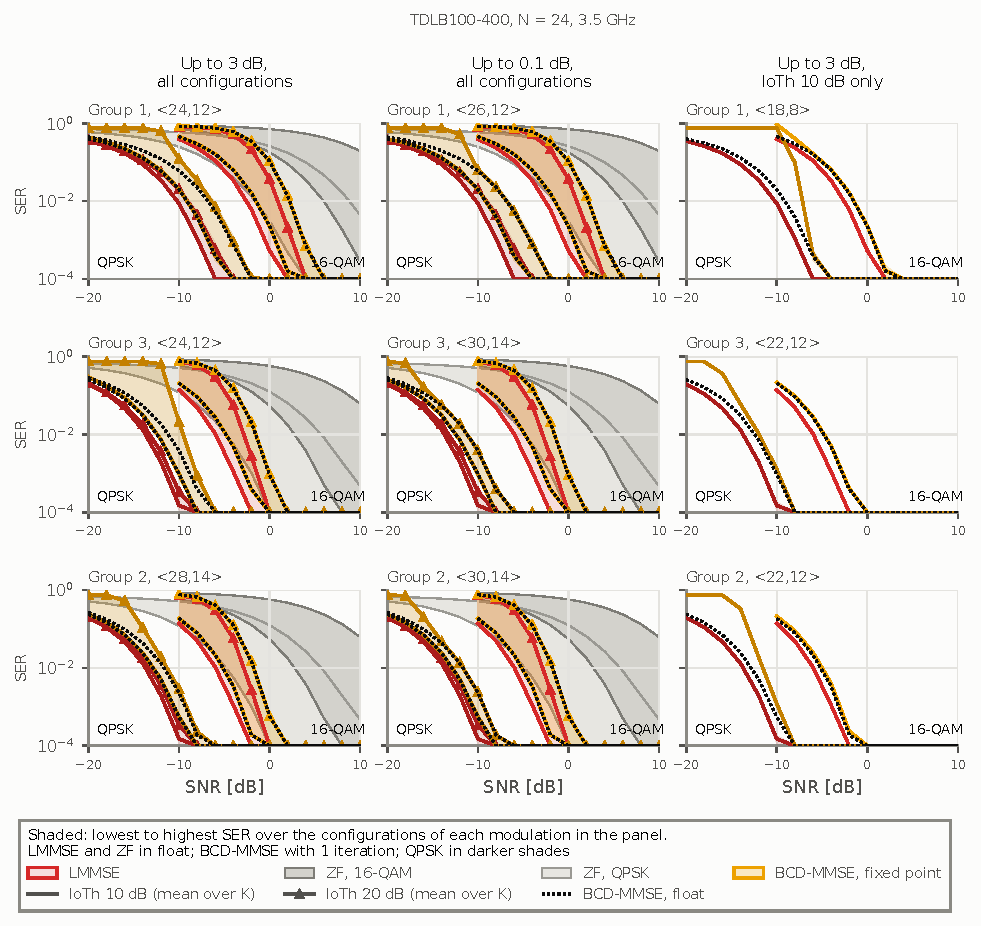
\includegraphics[width=\textwidth]{Images/RESULTADOS/curvas_ser/curvas_ser_grupos_range_B100.pdf}
\vspace{4pt}
\legend{\textcolor{red}{Fonte: a autora.}}
\end{figure}

\begin{figure}[!ht]
\caption{\textcolor{red}{Curvas de SER dos três grupos na TDLA30-5 e na TDLA30-10, nos formatos escolhidos.}}
\label{fig:curvas-range-a30}
\vspace{4pt} % a classe zera o espaço entre a caption e a figura
\centering
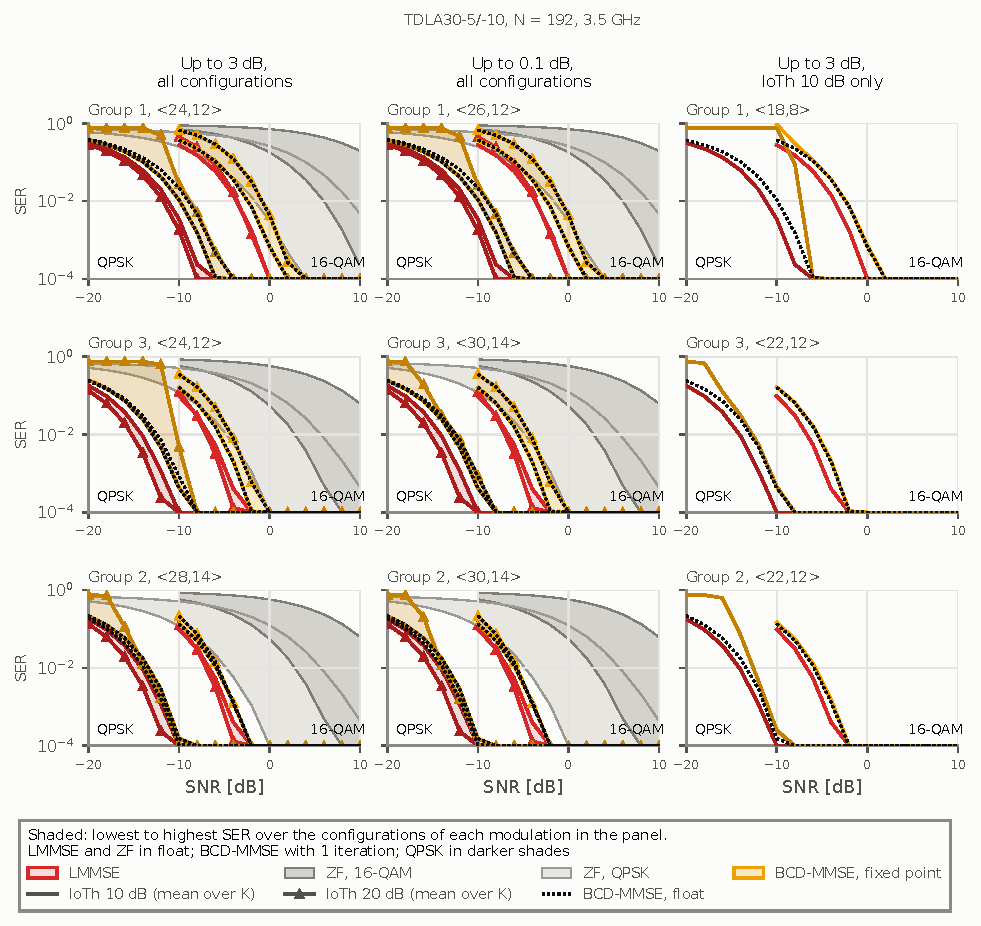
\includegraphics[width=\textwidth]{Images/RESULTADOS/curvas_ser/curvas_ser_grupos_range_A30-5.pdf}
\vspace{4pt}
\legend{\textcolor{red}{Fonte: a autora.}}
\end{figure}
